\newpage
\section{Grundlagen}
\label{sec:bdd_grundlagen}
Wie bereits in der Einleitung auf Seite \pageref{sec:einleitung} erwähnt, gibt es viele verschiedene Möglichkeiten, Boolesche Funktionen zu repräsentieren. Mithilfe von BDDs können Boolesche Funktionen effizient dargestellt werden. So können sie z.\,B. dazu eingesetzt werden, um große Primimplikantenmengen (siehe Kapitel \ref{sec:bAusdruecke} auf Seite \pageref{sec:bAusdruecke}) unter Verwendung der charakteristischen Funktion effizient darzustellen \cite[S.106-108]{ms1999}. Im Gegensatz dazu sind Normalformen wie bspw. die DNF oder KNF in der Praxis nur für sehr wenige Eingänge einsetzbar, da sehr viel Speicherplatz benötigt wird (siehe Kapitel \ref{sec:dnfknf} auf Seite \pageref{sec:dnfknf}). Formeln in KNF oder DNF lassen sich direkt in Second-Level Schaltungen realisieren, BDDs sind ein Beispiel für mehrstufige Schaltkreise (siehe Kapitel \ref{sec:bdd} auf Seite \pageref{sec:bdd}) bzw. eine Datenstruktur für Logiksynthese und Verifikation, womit Entscheidungs- bzw. Berechnungsprobleme wie der Äquivalenztest oder die Synthese (siehe Kapitel \ref{sec:verifikation} ab Seite \pageref{sec:verifikation}) effizient lösbar sind.\\
Die Grundfrage ist dabei, welche Anforderungen an Datenstrukturen für Boolesche Funktionen gestellt werden. Bei der Verifikation bspw. soll für einen Schaltkreis überprüft werden, ob er eine gewünschte Funktion realisiert, die ebenfalls durch eine Spezifikation gegeben ist. Für beide Funktionen kann nun ein BDD berechnet werden, inklusive einer anschließenden Überprüfung auf Äquivalenz, wobei dieses Vorgehen -- wie auch der Tautologietest -- im Allgemeinen für Formeln als auch Schaltkreise co-NP-vollständig ist \cite[S.6]{s2007}. Die Erwartungshaltung sollte daher sein, dieses Verfahren für praktisch relevante Funktionen effizient durchführbar zu gestalten.\\
Insgesamt gesehen werden also viele verschiedene Anforderungen an Boolesche Funktionen gestellt, wobei die wichtigsten Operationen in Kapitel \ref{sec:operationen} ab Seite \pageref{sec:operationen} diskutiert werden.

\subsection{Formale Definitionen}
\label{sec:formal}
In dieser Arbeit werden verschiedene Operationen in Bezug auf Entscheidungs- bzw. Berechnungsprobleme algorithmisch realisiert als auch die Größenordnung der Rechenzeit angegeben, wobei ein Algorithmus die Beschreibung einer Methode zur Lösung eines Problems kennzeichnet. Die Fälle umfassen dabei den Worst-, Best- und Average Case.\\ Hierzu wird die sog. \emph{asymptotische Komplexität} benutzt, die den Aufwand in Abhängigkeit von der Größe der Eingabe angibt. Sei hierzu also $f : \mathbb{N} \rightarrow \mathbb{R}_0^+$ eine Funktion. Die Ordnung von $f$ ist die Menge $O(f(n)) = \{ t : \mathbb{N} \rightarrow \mathbb{R}_0^+ \mid \exists c \in \mathbb{R}^+ \exists n_0 \in \mathbb{N} \forall n \geq n_0 : t(n) \leq c \cdot f(n) \}$, die das Wachstum von $f$ charakterisiert, d.\,h. sie enthält alle Funktionen, deren Graph maximal so stark wächst wie der Graph von $f$. Es wird dabei im Wesentlichen die Zeitkomplexität (Anzahl der benötigten Programmschritte) betrachtet, da sie unmittelbar eine obere Schranke für die Platzkomplexität (Größe des benötigten Speicherplatzes) impliziert \cite[S.118]{mt1998}.
Eine Menge $M \subseteq \mathbb{R}$ heißt nach oben beschränkt, falls es ein $K \in \mathbb{R}$ gibt, sodass $x \leq K \forall x \in M$. $K$ heißt \emph{obere Schranke} von $M$. Die kleinste obere Schranke von $M$ wird als \emph{Supremum} bezeichnet. $M \subseteq \mathbb{R}$ heißt wiederum \emph{nach unten beschränkt}, falls es ein $k \in \mathbb{R}$ mit $x \geq K \forall x \in M$ gibt. Dabei wird $k$ als \emph{untere Schranke} von $M$ bezeichnet. Die kleinste untere Schranke von $M$ heißt \emph{Infimum}.\\
Allgemein betrachtet ist ein Entscheidungsproblem eine Abbildung $D : IN \rightarrow BOOL$. $D$ heißt \emph{entscheidbar}, falls eine Turingmaschine (TM) existiert, sodass sie in einem Endzustand stoppt, falls $D(x)=JA$, wobei $x \in IN$. Ansonsten hält sie in einem Nicht-Endzustand.\\
Es gilt $D \in NP$, falls die TM Polyzeit-beschränkt und nichtdeterministisch ist, d.\,h. es können zu jedem Berechnungszustand mehrere Folgezustände existieren. Sollte die TM Polyzeit-beschränkt und deterministisch sein, so gilt $D \in P$. $P$ und $NP$ kennzeichnen diesbezüglich Komplexitätsklassen. Viele Probleme sind darüber hinaus nicht nur in NP, sondern auch NP-hart, wodurch NP-Vollständigkeit gekennzeichnet ist. $D$ heißt NP-hart, falls $D' \geq_p D \forall D' \in NP$, wobei $\geq_p$ eine Polynomialzeitreduktion kennzeichnet. Es gilt also $D' \geq_p D$, falls es eine totale berechnende Funktion $trans : IN' \rightarrow IN$ mit polynomiell beschränkter Berechnungslänge gibt, sodass $D'(x)=JA \Leftrightarrow D(trans(x))=JA$. Es werden also alle Ja- bzw. Nein-Instanzen auf das andere Problem bei einer Reduktion abgebildet. Intuitiv gesagt sind Probleme, die NP-vollständig sind, wahrscheinlich nicht effizient lösbar.\\
Entscheidbarkeit ist weiterhin ein Spezialfall von Berechnungsproblemen, die als Funktionen $\mathbb{N}^k \rightarrow \mathbb{N}$ ($k$ sei die Stelligkeit) kodiert werden, wobei die Ausgabe eine Menge von Objekten ist.

\subsubsection{Boolesche Funktionen}
\label{sec:bFunktionen}
Sei $f \subseteq N \times M$ eine \emph{Relation}. Dann heißt $f$, falls $\forall x \in N, y,z \in M (x,y) \in f \wedge (x,z) \in f \Rightarrow y = z$ rechtseindeutig und $\forall x \in N \exists y \in M : (x,y) \in f$ linkstotal ist, \emph{Abbildung} von $N$ nach $M$. $N$ kennzeichnet die Quell- und $M$ die Zielmenge der Abbildung. Die Abbildung $f$ heißt \emph{injektiv}, falls $\forall x,y \in N : f(x) = f(y) \Rightarrow x = y$ und \emph{surjektiv}, falls $\forall y \in M \exists x \in N : f(x) = y$ besteht. Gelten beide Eigenschaften, so wird die Abbildung als \emph{bijektiv} bezeichnet. Sei $A \subseteq N$, dann heißt $f(A) = \{ f(x) \mid x \in A \}$ \emph{Bild} von $A$. Ist $B \subseteq M$, dann heißt $f^{-1}(B) = \{ x \in N \mid f(x) \in B \}$ \emph{Urbildmenge} von $B$.\\
Abbildungen $f: \{0, 1\}^n \rightarrow \{0, 1\}^m$ ($n,m \in \mathbb{N}$) werden als \emph{Boolesche Funktionen} bezeichnet. Für die Eigenschaften gilt:
\begin{itemize}
	\item $(\mathbb{B}^n, f)$ heißt \emph{vollständig}, gdw. $f$ surjektiv ist.
	\item $(\mathbb{B}^n, f)$ heißt \emph{eindeutig}, gdw. $f$ injektiv ist.
	\item $(\mathbb{B}^n, f)$ heißt \emph{kanonisch}, gdw. $f$ bijektiv ist.
	\item $(\mathbb{B}^n, f)$ heißt \emph{operationell abgeschlossen}, gdw. $\forall a,b \in \mathbb{B}^n$ $\exists$ Darstellungen $u,v,w \in \mathbb{B}^n$ mit
	\begin{itemize}
		\item $f(u) = f(a) \cdot f(b)$
		\item $f(v) = f(a) + f(b)$
		\item $f(w) = f(a)'$
	\end{itemize}
\end{itemize}
$\mathbb{B}_{n,m}$ beschreibt die Menge aller Booleschen Funktionen von $\mathbb{B}^n \rightarrow \mathbb{B}^m$. Eine Abbildung $f : D \rightarrow \mathbb{B}^m, D \subset \mathbb{B}^n$ heißt \emph{(partielle) Boolesche Funktion} in $n$ Variablen. Sei $m=1$, dann gilt $ON(f) := \{ x \in \{0,1 \} \mid f(x) = 1 \}$ (Erfüllbarkeitsmenge) und $OFF(f) := \{ x \in \{0,1 \} \mid f(x) = 0 \}$ (Nichterfüllbarkeitsmenge). Ist $f$ eine partielle Boolesche Funktion, so bezeichnet $def(f) := \{ x \in \{ 0, 1 \}^n \mid f(x) \text{ definiert}\}$ den \emph{Definitionsbereich} von $f$. Hingegen kennzeichnet $dc(f) := \{ x \in \{ 0, 1 \}^n \mid f(x) \text{ nicht definiert}\}$ den \emph{don't care-Bereich} von $f$.\\
Weiterhin werden Boolesche Funktionen $f \in \mathbb{B}_{n,m}$ als $m$-dimensionale Vektoren \\$(f_1, \dots, f_m)$ Boolescher Funktionen $f_i \in \mathbb{B}_n, 1 \leq i \leq m$ aufgefasst.\\
Eine Boolesche Funktion $f(x_1, \dots, x_n)$ heißt genau dann \emph{symmetrisch}, wenn der Funktionswert durch einen Vektor $w = (w_0, \dots, w_n), w_i \in \{ 0,1 \}$ angegeben werden kann, wobei $w_i = 1 \Leftrightarrow f(a_1, \dots, a_n) = 1$ und $|\{a_j, j =1 \dots n : a_j = 1 \}| = i$. Der Funktionswert ist also nur von der Anzahl der Einsen im Argument, nicht aber von deren Position abhängig.\\
Hinsichtlich der Eigenschaften gibt es insgesamt $2^{m \cdot 2^n}$ Boolesche Funktionen in $B_{n,m}$ und $2^{2^n}$ Boolesche Funktionen in $\mathbb{B}_n$, wobei wenige davon -- die wenigstens $2^{n-1}$ Bits zur Darstellung in einer beliebigen Form benötigen -- exponentiell gegen $1$ für $n \rightarrow \infty$ konvergieren \cite[S.17]{h2002}. Es kann also nur erreicht werden, dass möglichst viele praktisch relevante Funktionen kompakt darstellbar sind (siehe Kapitel \ref{sec:bdd_grundlagen} auf Seite \pageref{sec:bdd_grundlagen}).
\subsubsection{Boolesche Ausdrücke}
\label{sec:bAusdruecke}
Boolesche Funktionen können in Form von \emph{Booleschen Ausdrücken} dargestellt werden, die auf den Regeln der \emph{Booleschen Algebra} basieren. Sei hierzu $M$ eine endliche Menge, auf der zwei binäre Operationen $\cdot, +$ und eine unäre Operation $\sim$ definiert sind. Das Quadrupel $(M, \cdot, +, \sim)$ heißt Boolesche Algebra, falls $\forall x, y, z \in M$ die folgenden Axiome gelten:
\begin{itemize}
	\item Kommutativität: $x+y = y+x$ sowie $x \cdot y = y \cdot x$
	\item Assoziativität: $x+(y+z) = (x+y)+z$ sowie $x\cdot(y\cdot z) = (x \cdot y) \cdot z$
	\item Distributivität: $x + (y \cdot z) = (x+y) \cdot (x+z)$ sowie $x \cdot (y+z) = (x \cdot y) + (x \cdot z)$
	\item Absorption: $x+(x \cdot y) = x$ sowie $x \cdot (x+y) = x$
	\item Auslöschung: $x+(y\cdot \sim y) = x$ sowie $x \cdot(y+\sim y) = x$
\end{itemize}
Viele weitere Gesetze wie bspw. die \emph{De Morganschen Gesetze} $~(x+y) = \sim x \cdot \sim y$ sowie $\sim(x \cdot y) = \sim x + \sim y$ sind zudem aus diesen Axiomen ableitbar.\\
Auf Basis dieser Regeln können nun Boolesche Ausdrücke definiert werden. Sei hierzu $A = X_n \cup \{ 0, 1, +, \cdot, \sim, (,) \}$ ein Alphabet, wobei $X_n = \{ x_1, \dots, x_n \}$ und $n \in \mathbb{N}$ gilt. Die Menge $BE(X_n)$ ist eine Teilmenge von $A^*$, die wie folgt induktiv definiert ist:
\begin{itemize}
	\item $0, 1, x_1, \dots, x_n$ sind Boolesche Ausdrücke.
	\item Sind $g$ und $h$ Boolesche Ausdrücke, so auch die Disjunktion ($+$ bzw. $\vee$), Konjunktion ($\cdot$ bzw. $\wedge$) und Negation $(\sim bzw. \neg)$.
\end{itemize}
Darüber hinaus gilt $\vee < \wedge < \neg$, d.\,h. z.\,B. hat die Negation eine höhere Präzedenz als die Konjunktion. Boolesche Ausdrücke sind eine vollständige Darstellung von $\mathbb{B}_n$, jedoch sind sie nicht eindeutig. Jedem Booleschen Ausdruck kann ein \emph{Operatorbaum} (siehe Abbildung \ref{fig:obaum}) zugeordnet werden, der zu jedem Ausdruck angibt, wie er korrekt ausgewertet werden kann:
\begin{figure}[bth]
	\centering
	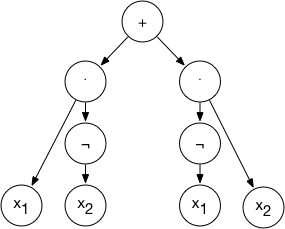
\includegraphics[scale=0.5]{./img/obaum}
	\caption[Operatorbaum für $(x_1\neg x_2)+(\neg x_1x_2)$]{Operatorbaum für $(x_1\neg x_2)+(\neg x_1x_2)$}
	\label{fig:obaum}
\end{figure}\\
\noindent
Bezüglich der Interpretation Boolescher Ausdrücke definiert also jeder Ausdruck eine Boolesche Funktion $\gamma : BE(X_n) \rightarrow \mathbb{B}_n$, wobei $\gamma(0) = 0$ sowie $\gamma(1) = 1$, d.\,h. $\forall x \in \mathbb{B}^n$ gilt:
\begin{itemize}
	\item $\gamma((g + h)) = \gamma(g) + \gamma(h)$
	\item $\gamma((g \cdot h)) = \gamma(g) \cdot \gamma(h)$
	\item $\gamma((\sim g)) = \sim \gamma(g)$
\end{itemize}
Die Booleschen Ausdrücke $x_i, x_i'$ heißen \emph{Literale}. Ein \emph{Monom} ist eine Konjunktion von Literalen und wird als \emph{Minterm} $m$ bezeichnet, falls $m(a) = \prod_{i=1}^{n}x_i^{a_i}$, wobei $a \in \mathbb{B}^n$. Die Disjunktion von paarweise verschiedenen Monomen wird als \emph{Polynom} bezeichnet, d.\,h. $f = \sum_{a \in ON(f)}m(a)$, wobei $a \in \mathbb{B}^n$. Die primären Kosten sind gleich der Anzahl der Monome in $f$. Die sekundären Kosten hingegen sind gleich der Anzahl der Literale in Addition zu der Anzahl der Monome in $f$. Ein \emph{Implikant} einer Booleschen Funktion $g$ ist ein Monom $q$ mit $\gamma(q) \leq g$ und ein \emph{Primimplikant} von $g$ ist ein maximaler Implikant $g$, d.\,h. er ist in keinem anderen Implikanten vollständig enthalten. Zwei Boolesche Ausdrücke $e_1, e_2$ sind darüber hinaus äquivalent, wenn $\gamma(e_1) = \gamma(e_2)$ gilt.
\subsubsection{Disjunktive und konjunktive Normalform}
\label{sec:dnfknf}
Die DNF bzw. KNF repräsentieren eine Boolesche Funktion $f \in \mathbb{B}_n$ als Summe von Produkten bzw. Produkt von Summen mittels $f(x) = \bigvee_{a \in f^{-1}(1)}m_a(x)$ respektive\\ $\bigwedge_{a \in f^{-1}(0)}s_a(x)$, wobei $s_a(x) = \bigvee_{i=1}^n x_i^{\overline{a_i}}$ (Maxterm) und $m_a(x) = \bigwedge_{i=1}^n x_i^{a_i}$ (Minterm). Die DNF ist kanonisch durch die Disjunktion aller Minterme. Hingegen wird die KNF durch die Konjunktion aller Maxterme als kanonisch bezeichnet. Diesbezügliche Beispiele sind im Zusammenhang mit BDDs in Kapitel \ref{sec:beispiele} auf Seite \pageref{sec:beispiele} zu finden.\\
Es sei erwähnt, dass durch diese Darstellung einige Nachteile auftreten. So haben viele intuitiv einfache Boolesche Funktionen, wie etwa die Paritätsfunktion $f_n = x_1 \oplus x_2 \oplus \dots \oplus x_n$ auf $n$ Variablen, damit eine exponentielle Darstellung. Diese symmetrische Funktion liefert $1$, wenn eine ungerade Anzahl von Eingängen den Wert $1$ besitzen, ansonsten gibt sie $0$ zurück. Hinsichtlich der Darstellung als DNF/KNF würde es $2^{n-1}$ Min- bzw. Maxterme geben \cite[S.21]{h2002}.

\subsubsection{Wahrheitstafeln}
\label{sec:wahrheitstafeln}
Ein Bitstring $b[0 : 2^n - 1]$ kann durch die Boolesche Funktion $f(b)(x) = b \left[ \sum_{i=0}^{n-1} x_i 2^i \right] \forall x \\\in \mathbb{B}^n]$, wobei $f(b) \in \mathbb{B}_n$, interpretiert werden. Dieser Bitstring heißt \emph{Wahrheitstafel} der Booleschen Funktion $f(b)$. Bitstrings der Länge $2^n$ sind zusammen mit dieser Interpretation als Boolesche Funktionen kanonische Darstellungen von $\mathbb{B}_n$. Im Zusammenhang mit BDDs ist ein Beispiel dazu in Kapitel \ref{sec:beispiele} auf Seite \pageref{sec:beispiele} ersichtlich.

\subsubsection{Schaltkreise}
\label{sec:schaltkreise}
Jedem Schaltkreis eine Boolesche Funktion zugeordnet werden, was auch umgekehrt gilt \cite{r2007}. Die Berechnung einer solchen Funktion wird als \emph{Simulation} bezeichnet, was in Kapitel \ref{sec:verifikation} auf Seite \pageref{sec:verifikation} beim Äquivalenztest demonstriert wird. Ein \emph{Schaltkreis} oder \emph{logisches Netzwerk} $SK = (X_n, G, typ, in, out, Y_m)$ ist ein gerichteter Graph über $STD := \{ \neg, \wedge, \vee, \oplus, \Leftrightarrow, NAND, NOR \}$, wobei:
\begin{itemize}
	\item $G=(V, E)$ zykelfrei
	\item $X_n := (x_1, \dots, x_n)$ primäre Eingänge
	\item $Y_m := (y_1, \dots, y_m)$ primäre Ausgänge
	\item $in : V \backslash S \rightarrow S^*, in(m) \in S^{indeg(m)}$ Eingänge
	\item $out : V \backslash S \rightarrow S^*, out(m) \in S^{outdeg(m)}$ Ausgänge
	\item $(\{ 0,1 \} \cup X_n \cup Y_m) \subset V$ konstante Signale
\end{itemize}
Die Kosten entsprechen der Anzahl der Modulknoten $C(SK)$ und die Tiefe  $depth(SK)$ wird durch die Anzahl der Modulknoten auf dem längsten Pfad von einem primären Eingang zu einem primären Ausgang beschrieben. Die Darstellung über logische Netzwerke ist vollständig, aber nicht eindeutig.\\
Ein \emph{Pfad} bzw. \emph{Weg} von $v$ nach $v'$ der Länge $n$ ($n \in \mathbb{N}$) in $G$ ist eine alternierende Knoten-Kanten-Folge $p = v_0e_1v_1e_2\dots e_nv_n$ mit:
\begin{itemize}
	\item $v_0, \dots, v_n \in V$
	\item $e_1, \dots, e_n \in E$
	\item $v = v_0$
	\item $v' = v_n$
\end{itemize}
Insbesondere sei noch einmal hervorgehoben, dass der Schaltkreis kreisfrei ist, d.\,h. es gilt zusätzlich $v_0 \neq v_n$. In Kapitel \ref{sec:bdd} auf Seite \pageref{sec:bdd} sind diesbezüglich Beispiele in Form von Multiplexern zu finden.
\subsubsection{Binäre Entscheidungsdiagramme (BDDs)}
\label{sec:bdd}
Ein \emph{BDD} ist ein gerichteter, azyklischer Graph bzw. Baum $G = (V \cup \Phi \cup \{1\},E)$, der eine Boolesche Funktion repräsentiert sowie kreisfrei und zusammenhängend ist. Seine Knoten sind in drei Untermengen unterteilt. $V$ ist die Menge aller internen Knoten. Diese Knoten haben je zwei ausgehende Kanten. Jeder Knoten $v \in V$ besitzt eine Bezeichnung $l(v) \in S_F$, wobei $S_F = \{x_1, \dots, x_n\}$ die Menge der Variablen ist, von denen $f$ abhängt. $|f|$ kennzeichnet die Knotenanzahl unterhalb von $f$, $f'$ sei die Negation von $f$. Das $1$-Blatt ist der Endknoten, das keine ausgehenden Kanten besitzt. $\Phi$ ist die Menge der Funktionsknoten, die in einer eindeutigen Beziehung zu den Komponenten von $f$ stehen. Diese haben keine eingehenden Kanten und je nur eine ausgehende Kante. Die ausgehenden Kanten von den Funktionsknoten können die Eigenschaft des Komplements besitzen. Die ausgehenden Kanten von einem internen Knoten werden mit $t$ und $e$ (komplementierend) bezeichnet. Mit dem \emph{Tripel} $(l(v), t, e)$ wird ein interner Knoten und seine beiden ausgehenden Kanten bezeichnet, wobei $l(v)$ die \emph{Entscheidungsvariable} darstellt. Dieses bestimmt dabei $f$ eindeutig. Die \emph{top-Variable} eines Knotens $f$ sei die Variable, nach der $f$ zerlegt wurde. Wird eine Menge von Knoten betrachtet, so ist sie das Minimum der top-Variablen der einzelnen Knoten, d.\,h. $top(l(v), t, e) = min \{ top(f), top(t), top(e) \}$. Der Knoten zur eigentlichen Repräsentation wird \emph{Formel} genannt. Die Variablen in $S_F$ sind geordnet. Ist der Knoten $v_j$ ein Nachfolger des Knotens $v_i$, dann ist $l(v_i) < l(v_j)$. Für die repräsentierte Funktion gilt:
\begin{enumerate}
	\item Die Funktion des Endknotens ist die konstante Funktion $1$.
	\item Ist die Kante kein Komplement, so ist die Funktion einer Kante die Funktion des Knotens, auf den sie zeigt. Ansonsten ist die Funktion der Kante das Komplement der Funktion des Zielknotens.
	\item Die Funktion eines internen Knotens $v \in V$ ist gegeben durch $(l(v) \wedge f_t) \vee (\neg l(v) \wedge f_e)$ (Shannon-Zerlegung), wobei $f_t, f_e$ die Funktionen der Kanten $(t, e)$ von $v$ sind. Die Funktion wird also mit Kofaktoren dargestellt.
	\item Die Funktionen des Funktionsknotens $\phi \in \Phi$ ist die Funktion der davon ausgehenden Kante.
\end{enumerate}
Wichtige Komplexitätsmaße für BDDs sind die Größe, d.\,h. die Anzahl der inneren Knoten sowie die Tiefe zur Kennzeichnung des längsten Pfades von der Wurzel zu einem Blatt.\\
BDDs lassen sich weiterhin unmittelbar durch ein Multiplexer-Netzwerk (Selektionsschaltungen) realisieren \cite{adk1991}. Dabei wird ein BDD $1:1$ in Schaltungsstrukturen umgesetzt, die aus $2:1$-Multiplexern bestehen, was die Abbildung \ref{fig:bddToMux} zeigt:
\begin{figure}[bth]
	\centering
	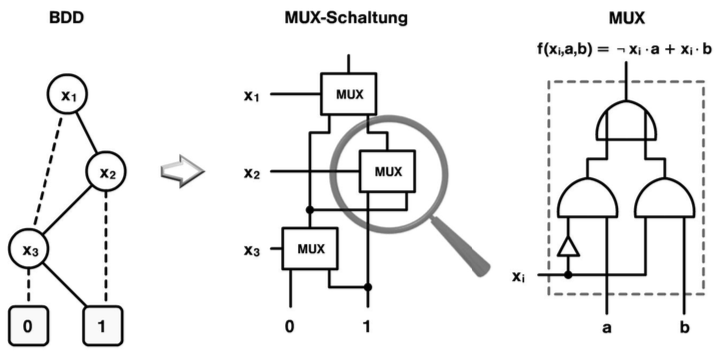
\includegraphics[scale=0.4]{./img/mux}
	\caption[BDD zu Multiplexer]{BDD zu Multiplexer \cite[S.46]{h2002}}
	\label{fig:bddToMux}
\end{figure}
\noindent
Jeder Knoten steht für einen Multiplexer, wobei sie mittels einem Bottom-up Verfahren erzeugt werden. An der Wurzel ist demnach der Ausgang zu finden.\\
Allgemein schalten Multiplexer von vielen Eingängen auf einen Ausgang, d.\,h. es wird $mux_n : \mathbb{B}^{2n+1} \rightarrow \mathbb{B}^n$ berechnet, wobei:\\
$mux_n(a_{n-1}, \dots, a_0, b_{n-1}, \dots, b_0, x_i) = \begin{cases}(a_{n-1} \dots a_0)& x_i = 1 \\ (b_{n-1} \dots b_0) & x_i = 0 \end{cases}$\\
Die Kosten betragen $C(mux_n) = 3n+1$, für die Tiefe gilt $depth(mux_n) = 3$.\\
Kaskadierte $2:1$-Multiplexer mit $n$ Variablen an den Auswahl- oder Adresseingängen können zudem zu einem Multiplexer mit $n$ Adresseingängen und $2^n$ Dateneingängen zusammengefasst werden. Dieser entspricht einem Nur-Lese-Speicher (ROM) mit $2^n$ Bits, was eine Grundstruktur der Zellen von Field Programmable Gate Arrays (FPGAs) kennzeichnet, welche programmierbare integrierte Schaltungen (ICs) darstellen.\\
Unter bestimmten Voraussetzungen -- die nachfolgend (siehe Kapitel \ref{sec:ordnung} ab Seite \pageref{sec:ordnung}) genauer beschrieben werden -- sind BDDs kanonisch, d.\,h. dass die Repräsentation einer gegebenen Funktion eindeutig ist.
\subsection{Beispiele zu Darstellungen Boolescher Funktionen}
\label{sec:beispiele}
Nachfolgend zeigt die Abbildung \ref{fig:operations} nun Beispiele bekannter Boolescher Operationen $x_1 \wedge x_2$, $x_1 \vee x_2$ und $x_1 \oplus x_2$:
\begin{figure}[bth]
	\centering
	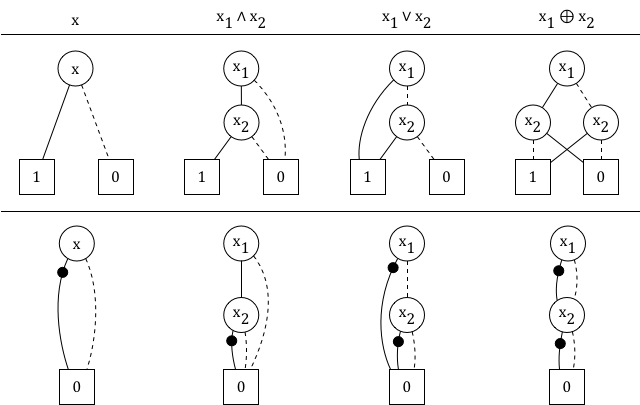
\includegraphics[scale=0.6]{./img/bdds}
	\caption[BDDs von bekannten Operationen]{BDDs von bekannten Operationen}
	\label{fig:operations}
\end{figure}\\
\textbf{Hinweis}: Zur Vereinfachung wurde der Startknoten $f$ weggelassen. Eine gestrichelte Linie entspricht der Kante $e$, eine durchgezogene Linie kennzeichnet hingegen die Kante $t$. Die ausgefüllten Kreise stehen wiederum für Output-Inverter hinsichtlich komplementärer Kanten, die in Kapitel \ref{sec:complementEdges} auf Seite \pageref{sec:complementEdges} beschrieben werden.\\
\\Um den Funktionswert zu einer gegebenen Variablenbelegung zu finden, muss (ausgehend vom Wurzelknoten) jedem Variablenknoten der $t$-Kante gefolgt werden, wenn die Variable den Wert $1$ hat, ansonsten der $e$-Kante, was einen Weg kennzeichnet (siehe Kapitel \ref{sec:schaltkreise} auf Seite \pageref{sec:schaltkreise}).\\
Wie bereits in der Definition \ref{sec:bdd} auf Seite \pageref{sec:bdd} erwähnt -- was hier gut zu beobachten ist -- gilt auch die Kreisfreiheit sowie der Zusammenhang, da $\exists$ ein Weg von $v$ nach $v'$ für je zwei Knoten $v, v' \in V$. Der erreichte Endknoten gibt dann den jeweiligen Funktionswert an. Letztendlich resultiert durch die Iteration eine sog. Wahrheitstafel (siehe Kapitel \ref{sec:wahrheitstafeln} auf Seite \pageref{sec:wahrheitstafeln}), die folgende Tabelle \ref{tab:wtabelle} darstellt:
\begin{table}[bth]
	\centering
	\caption{Wahrheitstabellen von bekannten Operationen}
	\label{tab:wtabelle}
	\begin{tabular}{ | c | c | c | c | c | }
		\hline
		\textbf{$x_1$} & \textbf{$x_2$} & \textbf{$x_1 \cdot x_2$} & \textbf{$x_1 + x_2$} & \textbf{$x_1 \oplus x_2$} \\ \hline
		$0$ & $0$ & $0$ & $0$ & $0$ \\ \hline
		$1$ & $0$ & $0$ & $1$ & $1$ \\ \hline
		$0$ & $1$ & $0$ & $1$ & $1$ \\ \hline
		$1$ & $1$ & $1$ & $1$ & $0$ \\ \hline
	\end{tabular}
\end{table}\\
\noindent
Der Bitstring $00$ entspricht somit z.\,B. dem Funktionswert $0$ bei $x_1x_2$. Anhand eines BDDs kann also auch eine DNF bzw. KNF abgeleitet werden. Gemäß der Definition aus Kapitel \ref{sec:dnfknf} auf Seite \pageref{sec:dnfknf} wäre somit bspw. die DNF von $x_1 \oplus x_2$ $(x_1\neg x_2) + (\neg x_1 x_2)$. Die KNF wäre durch $(x_1 + x_2) \cdot (\neg x_1 \neg x_2)$ bestimmt.\\
Hinzuzufügen ist, dass die negierte Funktion die gleiche Struktur hat, es sind lediglich die Einsen und Nullen der Wertzuweisungen vertauscht, was in Kapitel \ref{sec:implementierung} auf Seite \pageref{sec:implementierung} weitergehend erläutert wird.
\subsection{Reduzierte geordnete BDDs (ROBDDs)}
\label{sec:ordnung}
Ein Entscheidungsdiagramm (DD) heißt \emph{frei}, wenn es auf jedem Pfad von der Wurzel zu einem Blatt jede Variable höchstens einmal als Markierung vorkommt. Es heißt wiederum \emph{geordnet}, wenn auf jedem Pfad von der Wurzel zu einem Blatt die Variablen in der gleichen Reihenfolge abgefragt werden:
\begin{figure}[bth]
	\centering
	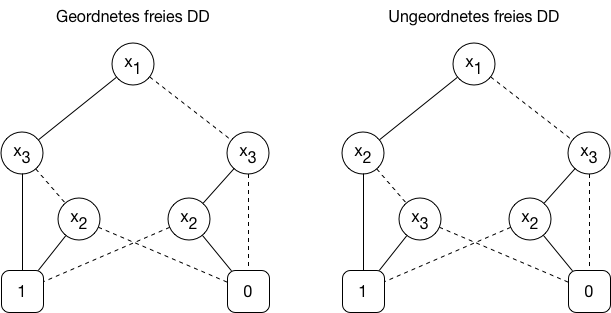
\includegraphics[scale=0.5]{./img/ordnung}
	\caption[Geordnetes und ungeordnetes freies DD]{Geordnetes und ungeordnetes freies DD}
	\label{fig:ordnung}
\end{figure}\\
\noindent
Bei beiden Diagrammen aus der Abbildung \ref{fig:ordnung} geht hervor, dass sie frei sind, da auf jedem Pfad jede Variable höchstens einmal vorkommt. Das zweite Diagramm ist allerdings ungeordnet, da dort die Variablen nicht in der gleichen Reihenfolge abgefragt werden.\\
Eine Boolesche Funktion ist von $n$ Variablen abhängig, was für ein BDD bedeutet, dass er mindestens $2^{n+1}-1$ Knoten hat. Wie bereits in der Einleitung auf Seite \pageref{sec:einleitung} erwähnt, sollen Informationen aber kompakt dargestellt werden. Es kann vorkommen, dass sich beim Erstellen eines BDDs identische Kofaktoren ergeben, d.\,h. es gibt zwei interne Knoten, die dieselbe Funktion repräsentieren. Es kann aber auch passieren, dass redundante Knoten auftreten. Ein Knoten ist genau dann redundant, wenn seine t- als auch seine e-Kante auf denselben nächsten Knoten zeigen. Ein BDD heißt also \emph{reduziert}, wenn es keinen nichtterminalen Knoten $v$ mit dem Index $x$ und $(f_v)_x = (f_v)_x'$ gibt und auch keine verschiedenen Knoten $v, w$ existieren, die gleich markiert  sowie deren Kinder (falls vorhanden) jeweils identisch sind. Sowohl die Isomorphie- als auch die Redundanz-Regel sind in der Abbildung \ref{fig:reduziert} ersichtlich:
\begin{figure}[bth]
	\centering
	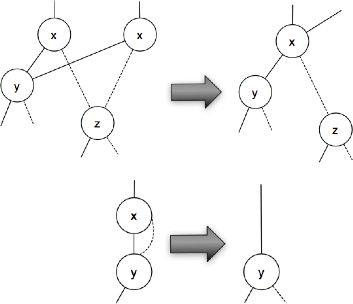
\includegraphics[scale=1.0]{./img/reduziert}
	\caption[Reduktionsregeln bei BDDs]{Reduktionsregeln bei BDDs}
	\label{fig:reduziert}
\end{figure}\\
\noindent
Durch die wiederholte Verschmelzung von isomorphen Teilgraphen und Entfernen redundanter Knoten entsteht letztendlich ein reduziertes BDD, was anhand der Abbildung \ref{fig:reduktionen} demonstriert wird:
\begin{figure}[bth]
	\centering
	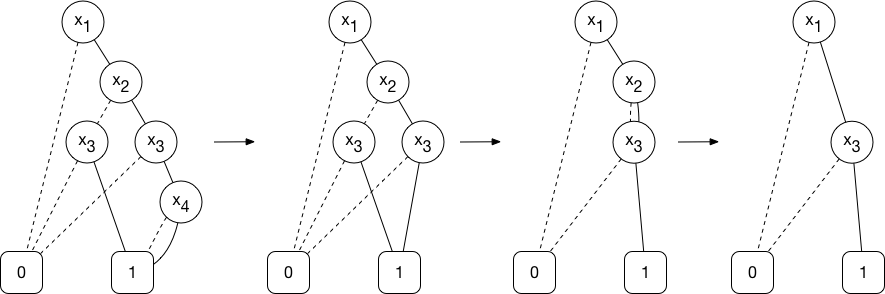
\includegraphics[scale=0.4]{./img/reduktionen}
	\caption[Anwendung der Reduktionsregeln bei einem BDD]{Anwendung der Reduktionsregeln bei einem BDD}
	\label{fig:reduktionen}
\end{figure}\\
\noindent
Hier gehen besonders die Abhängigkeiten der Regeln hervor. So ist gelegentlich erst eine Regel nach vorherigen Reduktionsschritten anwendbar. Insgesamt gesehen genügt es, solange Reduktionsregeln anzuwenden, bis keine Regel mehr anwendbar ist. Es sollte jedoch verhindert werden, dass zu häufig für einen Knoten geprüft wird, ob eine Regel angewendet werden kann. Es empfiehlt sich hier ein rekursiver Algorithmus, da so für Knoten endgültig entschieden werden kann, ob sie gelöscht oder mit einem anderen Knoten verschmolzen werden. Diese Frage stellt sich genau dann, wenn auf die Nachfolger keine Regel mehr angewendet werden kann \cite{a2010}:
\lstset{language=xml}
\begin{lstlisting}[frame=htrbl, caption={Implementierung von {\ttfamily reduce}}, label={lst:reduce}]
program reduce()
  input: OBDD G in Bezug auf f mit der Ordnung x[1], ..., x[n]
  output: ROBDD G'
  v := Innerer Knoten von g
  l0 := 0-Blatt
  l1 := 1-Blatt
  v.id := Nummer von v
  id := Nummer
  v.i := Index der Variablen, mit der v markiert ist
  v.low := low-Kind
  v.high := high-Kind
  vec := Liste, welcher Knoten die weiteren Nummern darstellt
  x := Markierte Knoten
  marked := Liste mit markierten Knoten
  foreach (G) do
    merge(l0.all)
    merge(l1.all)
    l0.id := 0
    vec[l0.id] := l0
    l1.id := 1
    vec[l1.id] := l1
    marked := (x[1], ..., x[n])
  end foreach
  id := 1
  for (i := n to 1) do
    while (marked) do
      if (v.low.id = v.high.id) then
        v.id := v.low.id
        marked.del(v)
      end if
    end while
    // Key von v ist (v.low.id, v.high.id)
    sort_lex(marked)
    // Verschmelze hintereinander stehende Knoten
    foreach (marked) do
      id := id + 1
      v[1].id := id
      vec[v[1].id] := v[1]
      v[1].0 := vec[v[1].low.id]
      v[1].1 := vec[v[1].high.id]
      v[2].id := v[1].id
      ...
      v[l].id := v[1].id
    end foreach
  end for
end program
\end{lstlisting}
Gemäß dem Code \ref{lst:reduce} können Knoten des OBDDs nicht direkt gelöscht werden, da es keine rückwärts gerichteten Zeiger gibt. Wenn also ein Knoten gelöscht werden soll, so müssen die Zeiger von $v$ auf den Nachfolger davon umgesetzt werden. Wenn die Knoten $v, w$ verschmolzen werden sollen, so müssen die Zeiger wiederum von $v$ auf $w$ umgelegt werden. Hier wird das Löschen derartig realisiert, indem $v$ die $id$ von $w$ erhält. Aufgrund dessen, dass nun mehrere Knoten mit derselben Nummer existieren können, wird in einem Vektor $vec$ gespeichert, welcher Knoten mit der jeweiligen Nummer die Übrigen repräsentiert. Hervorzuheben -- in Bezug auf den Redundanztest -- ist, dass lediglich eine Traversierung durch das OBDD ausreicht, was durch die Eigenschaften von ROBDDs bedingt ist \cite[S.44]{s2007}. Wenn $G$ keinen mit $x_i$ markierten Knoten besitzt, so wird für $x_i=0, x_i=1$ derselbe Funktionswert berechnet. Demnach hängt $f$ aber nicht maßgeblich von $x_i$ ab, was automatisch auch für alle Subfunktionen gilt. Das ROBDD enthält somit auch keinen mit $x_i$ markierten Knoten. Sollte $f$ im Umkehrschluss maßgeblich von $x_i$ abhängen, so gilt $f_{x_i=0} \neq f_{x_i=1}$ und das ROBDD enthält einen mit $x_i$ markierten Knoten.\\
Bei Implementierungen (siehe Kapitel \ref{sec:ite} ab Seite \pageref{sec:ite}) wird direkt bei der Synthese darauf geachtet, dass Reduktionen unmittelbar bei der Erstellung von Knoten angewendet werden können, um mehrfache Traversierungen zu verhindern.\\
Alle Operationen -- bis auf das Sortieren -- benötigen pro Knoten nur eine konstante Zeit, d.\,h. $O(1)$. Für das Sortieren kann Bucketsort verwendet werden, womit in der Liste dann Knoten mit den gleichen Nachfolgern gefunden werden können \cite{a2010}. Bucketsort ist daher ein Sortierverfahren, das für bestimmte Werte-Verteilungen einer Eingabeliste wie folgt sortiert:
\begin{enumerate}
	\item Die Elemente werden auf die \glqq Buckets\grqq{} verteilt (Partitionierung).
	\item Jeder \glqq Bucket\grqq{} wird mit einem weiteren Sortierverfahren sortiert.
	\item Der Inhalt der sortierten \glqq Buckets\grqq{} wird konkateniert.
\end{enumerate}
Die Ausgabedaten werden also gesondert gespeichert, womit die Eingabedaten nicht überschrieben werden. Der gesamte Algorithmus benötigt dementsprechend dann eine lineare Rechenzeit.\\
Nach dem Satz von Bryant sind ROBDDs kanonische Darstellungen Boolescher Funktionen \cite[S.677-691]{b1986}. Als Beispiel soll hierzu im Folgenden die Funktion \\$f(x_1, x_2, x_3, x_4) = \neg x_1x_2+x_2(x_3+x_4)$ mit der Variablenordnung $\pi : x_1 < x_2 < x_3 < x_4$ dienen, die aus der Abbildung \ref{fig:robdd} hervorgeht. Die jeweilige Subfunktion infolge der Shannon-Zerlegung (siehe Kapitel \ref{sec:bdd} auf Seite \pageref{sec:bdd}) ist an den Knoten gekennzeichnet:
\begin{figure}[bth]
	\centering
	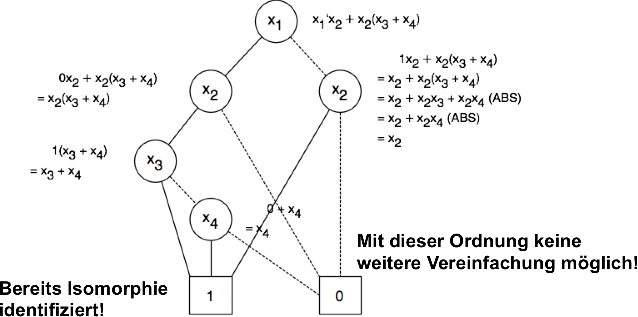
\includegraphics[scale=0.9]{./img/robdd}
	\caption[ROBDD für die Funktion $f = \neg x_1x_2+x_2(x_3+x_4)$]{ROBDD für die Funktion $f = \neg x_1x_2+x_2(x_3+x_4)$}
	\label{fig:robdd}
\end{figure}\\
\noindent
Diese Minimalitätsaussage bezieht sich jedoch nur auf eine Funktion $f$ mit fester Variablenordnung. Die nachfolgende Abbildung \ref{fig:robdd2} zeigt die Funktion $f$ mit einer anderen Variablenordnung $\pi : x_1 < x_3 < x_4 < x_2$:
\begin{figure}[bth]
	\centering
	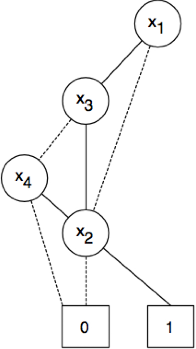
\includegraphics[scale=0.9]{./img/robdd2}
	\caption[ROBDD für $f$ mit einer anderen Ordnung]{ROBDD für $f$ mit einer anderen Ordnung}
	\label{fig:robdd2}
\end{figure}\\
\noindent
Die Größe hängt insgesamt von der Variablenordnung ab, die exponentiell sein kann \cite{p2010}. Zur Verdeutlichung dieses Sachverhalts wird die Funktion $f \in \mathbb{B}_{2n}$ mit \\
$f(x_1, x_2, x_3, x_4, \dots, x_{2n-1}, x_{2n}) = (x_1+x_2) (x_3+x_4)\dots(x_{2n-1}+x_{2n})$, wobei $n=3$ angenommen. Das dazugehörige ROBDD ist der Abbildung \ref{fig:expSize} auf Seite \pageref{fig:expSize} zu entnehmen:
\newpage
\begin{figure}[bth]
	\centering
	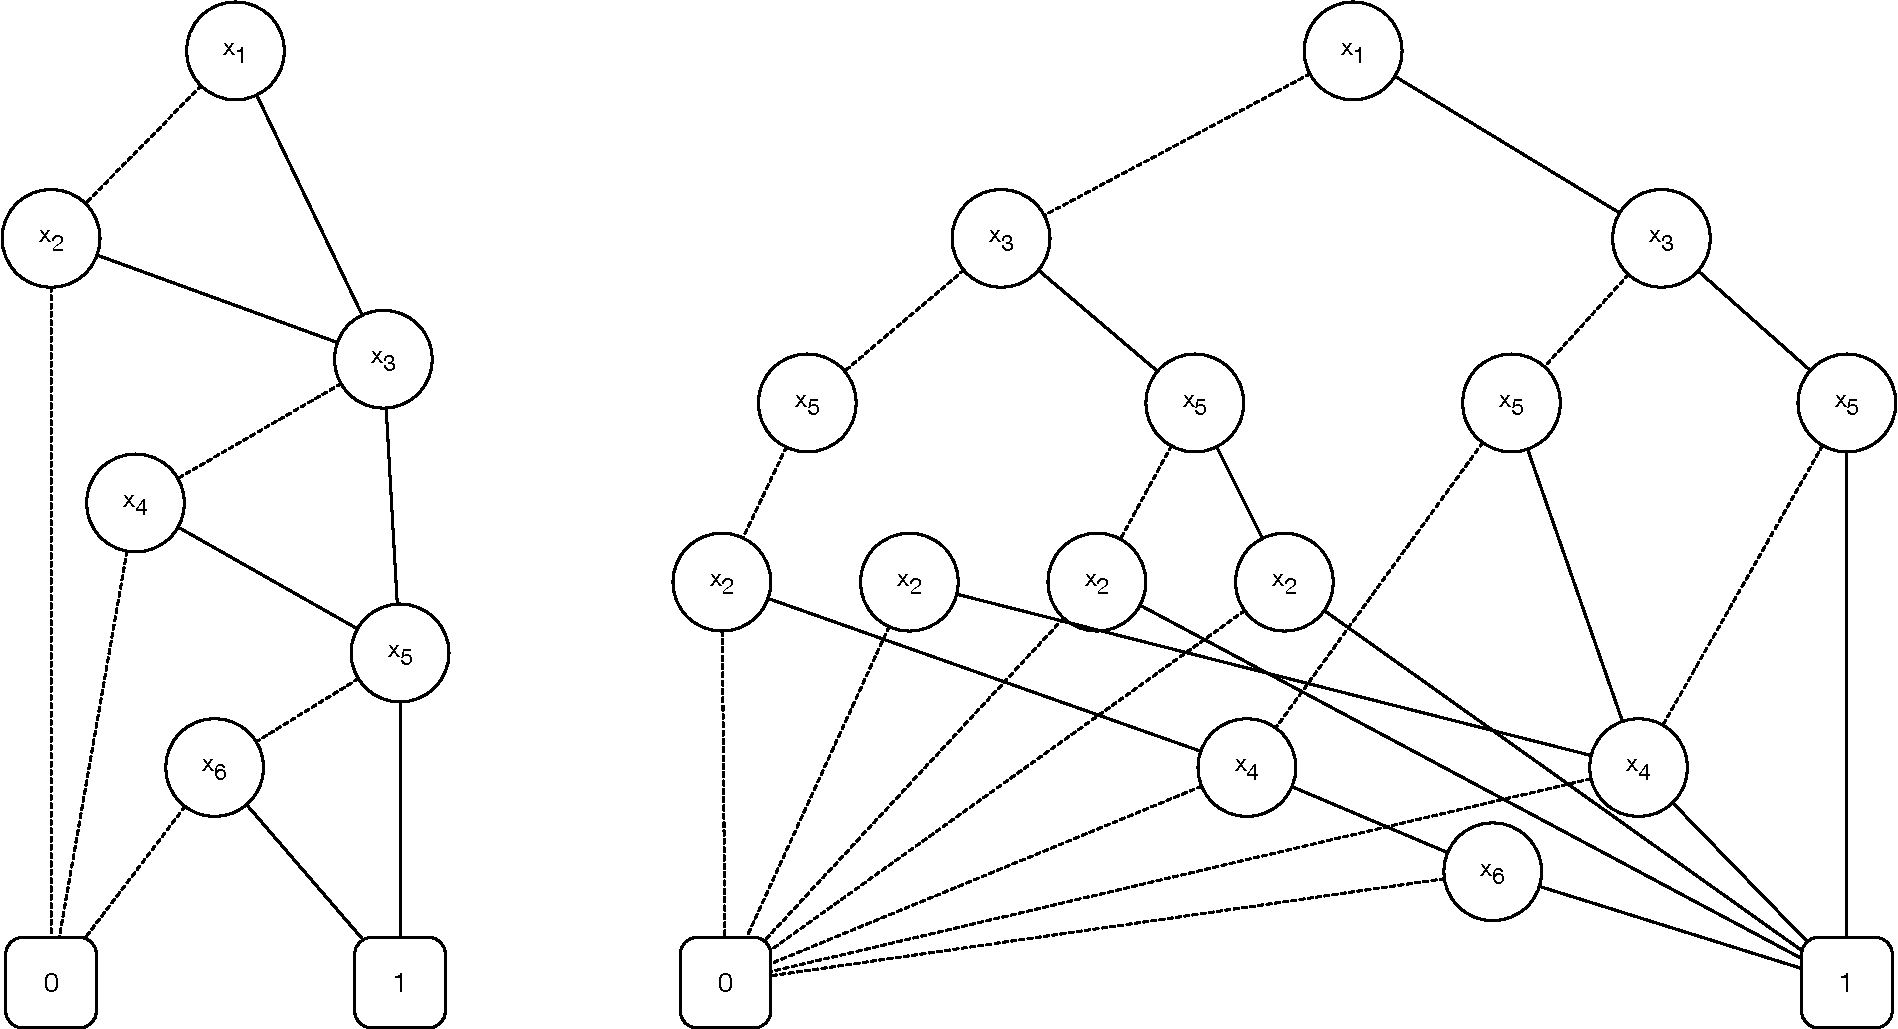
\includegraphics[scale=0.3]{./img/expSize}
	\caption[Lineares und exponentielles Wachstum von Knoten]{Lineares und exponentielles Wachstum von Knoten}
	\label{fig:expSize}
\end{figure}
Das linke ROBDD besitzt die Variablenordnung $\pi : x_1 < x_2 < x_3 < x_4 < x_5 < x_6$. Es ist zu erkennen, dass es sich hier um ein lineares Wachstum der Knoten in Bezug auf die Variablenanzahl handelt, da es $2n+2$ Knoten gibt. Wird hingegen die Variablenordnung $\pi : x_1 < x_3 < x_5 < x_2 < x_4 < x_6$ gewählt, so ist ein exponentielles Wachstum ersichtlich. Das ROBDD bläht sich hierzu bis zur Tiefe $n$ zu einem vollständig binären Baum auf, wobei jeder Knoten die Informationen zu allen vorherigen Variablenbelegungen besitzt. Somit können diese Knoten also nicht zusammengefasst werden und es gibt $2^{n+1}$ Knoten.\\
Eine gute Ordnung zu finden ist nicht immer leicht. So benötigen nahezu alle Booleschen Funktionen sogar mit einer optimalen Variablenordnung mindestens $\frac{2^n}{2n}$ Knoten \cite{ll92}. In der Praxis finden jedoch hauptsächlich Boolesche Funktionen eine Anwendung, die relativ einfach aufgebaut sind. Somit gelingt es i.\,d.\,R. eine optimale Ordnung zu finden, sodass eine Darstellung durch ein ROBDD effizient möglich ist \cite{g2002}. Insgesamt betrachtet ist das Problem, eine optimale Variablenordnung zu finden, jedoch NP-vollständig, kann allerdings mit verschiedenen Heuristiken in Polyzeit behandelt werden \cite{bw1999}.\\
Für viele Funktionen wie z.\,B. XOR liefern BDDs jedoch eine kompakte Repräsentation, selbst wenn sie mittels KNF/DNF nicht kompakt darstellbar sind. Es kann zudem in konstanter Zeit geprüft werden, ob eine Funktion (dargestellt durch ein BDD) erfüllbar (SAT), d.\,h. $sat(f) \Leftrightarrow \exists a \in B^n, \text{ sodass } f(a) = 1 \text{ für } f \in B_{n,1}$ (siehe Kapitel \ref{sec:erfuellbar} auf Seite \pageref{sec:erfuellbar}) oder eine Tautologie (siehe Kapitel \ref{sec:tautologietest} auf Seite \pageref{sec:tautologietest}) ist \cite{bfms2001}. Im Allgemeinen ist SAT nach dem Satz von Cook und Levin NP-vollständig, wobei die Laufzeit exponentiell ist, da alle $2^n$ Belegungen systematisch erzeugt werden müssen \cite{km2007}.
\subsection{Operationen auf BDDs}
\label{sec:operationen}
Wie bereits in Kapitel \ref{sec:bdd_grundlagen} auf Seite \pageref{sec:bdd_grundlagen} erwähnt, werden viele Anforderungen an Boolesche Funktionen gestellt.\\
Wenn Boolesche Funktionen realisiert bzw. analysiert werden, so wird auf Datenstrukturen gearbeitet, die als solche Funktionen interpretiert werden können. Mit ROBDDs sollen diesbezüglich praktisch wichtige Boolesche Funktionen effizient dargestellt und Berechnungen darauf ausgeführt werden. Besonders sollen effiziente Berechnungen ermöglicht werden, die mit anderen Darstellungen von Booleschen Funktionen wegen dem Bedarf der Rechenzeit und des Speicherplatzes nicht möglich sind. So gibt es bspw. den Äquivalenztest oder die Synthese, worunter ein Entscheidungs- bzw. Berechnungsproblem verstanden wird. Mithilfe von BDDs sind solche -- im Gegensatz zu Formeln oder Schaltkreisen -- effizient lösbar. Es sollen daher im Folgenden wichtige Operationen in ihrem Verfahren und ihrer Komplexität (siehe Kapitel \ref{sec:formal} auf Seite \pageref{sec:formal}) untersucht werden. So gibt es bspw. die Booleschen Operatoren wie \texttt{and}, \texttt{or} und \texttt{not}, die bezüglich ROBDDs in der Laufzeit polynomiell beschränkt sind, was in Kapitel \ref{sec:ite} auf Seite \pageref{sec:ite} gezeigt wird. Es können jedoch zu anderen Darstellungsformen Unterschiede festgestellt werden, die in der Tabelle \ref{tab:bop} erläutert sind \cite{m2007}:
\begin{table}[bth]
	\centering
	\caption{Vergleich der operationellen Komplexitäten für Darstellungen}
	\label{tab:bop}
	\begin{tabular}{ | l | p{10.5cm} | }
		\hline
		\textbf{Darstellung} & \textbf{Beschreibung} \\ \hline
		Wahrheitstafel & Die Laufzeit ist proportional zu $2^n$, d.\,h. linear in der Größe zur Wahrheitstafel.\\ \hline
		Boolesche Ausdrücke & Hierzu können die beiden Operatorbäume (siehe Kapitel \ref{sec:bAusdruecke} auf Seite \pageref{sec:bAusdruecke}) kopiert werden. Anschließend erfolgt eine Verknüpfung über eine neue Wurzel. Insgesamt besteht eine polynomielle Laufzeit. \\ \hline
		DNF & Die Or-Operation wird durch eine Konkatenation der DNFs umgesetzt, die And-Operation hingegen durch das Ausmultiplizieren davon. Diese Operation ist wie auch die Not-Operation, die durch Anwendung der Regel von De Morgan sowie anschließendem Ausmultiplizieren der Klauseln umgesetzt wird, recht teuer. Insgesamt besteht dennoch eine polynomielle Laufzeit. \\ \hline
		KNF & Hierbei sind die Or- und Not-Operation recht teuer. Die OR-Operation wird durch das Ausmultiplizieren der KNFs umgesetzt, die NOT-Operation hingegen durch Anwendung der Regel von De Morgan sowie anschließendem Ausmultiplizieren der Monome. Bei der And-Operation erfolgt lediglich eine Konkatenation der KNFs. Alle aufgeführten Operationen sind dabei polynomiell beschränkt. \\ \hline
		Schaltkreise & Die operationellen Komplexitäten entsprechen den Booleschen Ausdrücken. \\ \hline
	\end{tabular}
\end{table}\\
\noindent 
Auch Umwandlungen wie z.\,B. die Überführung einer KNF zu einer DNF kann die Formel exponentiell vergrößern, was nicht verhindert werden kann \cite{s2010}. Im Hinblick auf die verschiedenen Darstellungen gibt es im Laufzeitverhalten also bereits bei den Basisoperationen erhebliche Unterschiede. Weiterhin soll daher auch bezüglich weiterer nützlicher Operationen ein Vergleich zu anderen Darstellungen für Boolesche Funktionen gemacht werden. 

\subsubsection{Äquivalenztest}
\label{sec:verifikation}
Hardware- und Softwaresysteme finden eine immer größer werdende Verbreitung wie z.\,B. in eingebetteten Systemen wie Handys oder Autos. Zudem werden Systeme immer komplexer, was z.\,B. mit der Betriebssystementwicklung zusammenhängt \cite{b2008}. Aufgrund dessen, dass Fehler hohe Kosten verursachen, hat die Verifikation von Hardware- und Softwaresystemen eine enorme Bedeutung.\\
BDDs eignen sich -- wie bereits in Kapitel \ref{sec:bdd_grundlagen} auf Seite \pageref{sec:bdd_grundlagen} erwähnt -- zur Verifikation von Schaltungen. Eine zentrale Aufgabe dabei ist der sog. Äquivalenztest. Angenommen, es gibt zwei Schaltkreise, die in der Abbildung \ref{fig:sks} präsentiert werden:
\begin{figure}[bth]
	\centering
	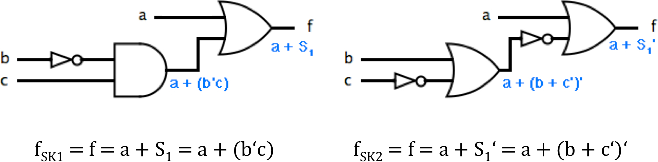
\includegraphics[scale=1.0]{./img/sks}
	\caption[Äquivalenz von Schaltkreisen]{Äquivalenz von Schaltkreisen}
	\label{fig:sks}
\end{figure}\\
\noindent
Mithilfe eines ROBDDs kann nun eine Aussage zur möglichen Äquivalenz dieser getroffen werden, indem es für die jeweiligen Schaltkreise erstellt wird. Die daraus resultierenden ROBDDs sind in Abbildung \ref{fig:aequivalenz} ersichtlich:
\begin{figure}[bth]
	\centering
	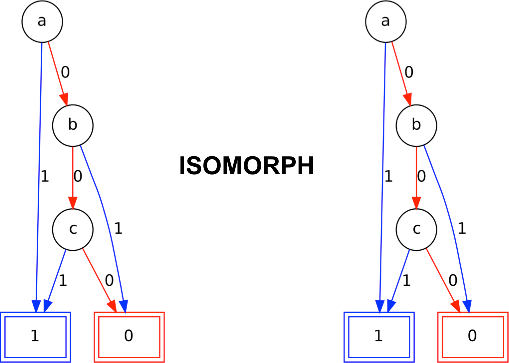
\includegraphics[scale=0.8]{./img/skbdds}
	\caption[Äquivalenztest mithilfe von BDDs]{Äquivalenztest mithilfe von BDDs}
	\label{fig:aequivalenz}
\end{figure}\\
Demnach sind beide Schaltkreise isomorph zueinander. Durch diesen Test können also unter anderem Schaltungen vereinfacht werden. Allgemein formuliert gilt also:\\
\begin{tabular}{l|p{12cm}}
	\textbf{Eingabe:} & OBDDs $G_a$ und $G_b$, wobei $a, b \in \mathbb{B}_n$. \\ 
	\textbf{Ausgabe:} & \texttt{JA}, falls $a = b$, \texttt{NEIN} sonst. \\ 
	\textbf{Verfahren:} & Es werden zunächst einmal $G_a$ und $G_b$ zu $G_a'$ und $G_b'$ reduziert. Anschließend werden $G_a'$ und $G_b'$ auf Isomorphie getestet.\\
	\textbf{Komplexität:} & $O(|G_a|+|G_b|)$, da die Reduktion sowie der Isomorphietest in linearer Zeit möglich sind, weil OBDDs Graphen mit einer Quelle und markierten Knoten sowie Kanten sind (siehe Kapitel \ref{sec:ordnung} auf Seite \pageref{sec:ordnung}). So können $G_a'$ und $G_b'$ simultan mit einer DFS durchlaufen werden, wobei getestet werden muss, ob die erreichten Knoten die gleiche Markierung haben.
\end{tabular}
Wenn $a$ und $b$ gemeinsam in einem reduzierten OBDD dargestellt werden bzw. in derselben Unique-Table (siehe Kapitel \ref{sec:utable} auf Seite \pageref{sec:utable}), so ist der Äquivalenztest in konstanter Zeit möglich. Es genügt hierbei der Test, ob die Zeiger für $a$ und $b$ auf denselben Knoten zeigen \cite[S.66]{ms1999}.\\
Bei Wahrheitstafeln hingegen ist die Laufzeit proportional zu $2^n$, d.\,h. linear in der Größe der Funktionstafeln. Bezüglich Booleschen Ausdrücken, der KNF/DNF und Schaltkreisen sind hierfür keine effizienten Verfahren bekannt.\footnote{Molitor, vgl.~\cite{m2007}}

\subsubsection{Auswertungsproblem}
\label{sec:auswertung}
Allgemein betrachtet ist hierzu eine Formel sowie eine Belegung gegeben und es stellt sich die Frage, ob diese Belegung zu einem Funktionswert von $1$ am Ausgang führt. Bezogen auf OBDDs gilt:\\
\begin{tabular}{l|p{12cm}}
	\textbf{Eingabe:} & OBDD $G$ für $f \in \mathbb{B}_n$, eine Belegung $x \in \{ 0, 1 \}^n$. \\ 
	\textbf{Ausgabe:} & \texttt{JA}, falls $f(x) = 1$, \texttt{NEIN} sonst. \\ 
	\textbf{Verfahren:} & Das OBDD wird von der Wurzel bis zu einem Blatt gemäß der Belegung durchlaufen. Anschließend wird die Markierung des erreichten Blattes ausgegeben. Dieser Vorgang wird auch als \emph{Evaluation} bezeichnet.\\
	\textbf{Komplexität:} & $O(n)$, da jede Variable höchstens einmal getestet werden darf. Bezüglich des Speicherplatzes gilt natürlich dennoch $O(|G|)$ für den dazugehörigen Aufbau.
\end{tabular}
\noindent
Hinzuzufügen ist, dass bei diesem Test nicht die Möglichkeit besteht, mithilfe eines ROBDDs für eine konstante Laufzeit zu sorgen, was durch folgende Abbildung \ref{fig:auswertung} auf Seite \pageref{fig:auswertung} verdeutlicht werden soll:
\newpage
\begin{figure}[bth]
	\centering
	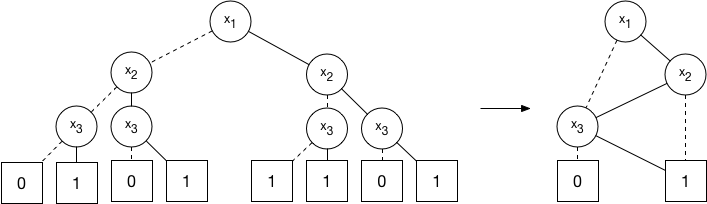
\includegraphics[scale=0.5]{./img/auswertung}
	\caption[BDDs zur Verdeutlichung des Auswertungsproblems]{BDDs zur Verdeutlichung des Auswertungsproblems}
	\label{fig:auswertung}
\end{figure}
Zu erkennen ist ein OBDD sowie ROBDD für die Boolesche Funktion $f(x_1, x_2, x_3) = x_1 \cdot \neg x_2 + x_3$, wobei $f \in \mathbb{B}_3$. Angenommen, die Belegung sei $x = (1,1,1)$, so würde die Funktion $1 \cdot 0 + 1$ zu $1$ auswerten. Bezüglich dem OBDD ist dies zu erkennen, indem gemäß des Verfahrens den Kanten entlang gelaufen wird. Hinsichtlich dem dazugehörigen ROBDD kann jedoch nicht anhand der Wurzel abgesehen werden, wie die Auswertung anhand der jeweiligen Belegung sein wird, da weiterhin die Variablen gemäß der Belegung abgelaufen werden müssen.\\
Im Vergleich zu den anderen Darstellungen für Boolesche Funktionen gilt ebenfalls ein linearer Aufwand, weil die Anzahl der Aufrufe zur Auswertung durch die Größe der Formel beschränkt ist \cite{m2007}.

\subsubsection{Erfüllbarkeit}
\label{sec:erfuellbar}
In Kapitel \ref{sec:ordnung} auf Seite \pageref{sec:ordnung} wurde erwähnt, dass durch die Kanonizität eines OBDDs der Erfüllbarkeitstest in konstanter Zeit möglich ist, was im Folgenden algorithmisch analysiert werden soll. Ein BDD ist erfüllbar, gdw. es nicht aus dem 0-Blatt besteht:\\
\begin{tabular}{l|p{12cm}}
	\textbf{Eingabe:} & OBDD $G$ für $f \in \mathbb{B}_n$. \\ 
	\textbf{Ausgabe:} & \texttt{JA}, falls $\exists$ eine Belegung $x \in \mathbb{B}^n : f_{G}(x) = 1$, \texttt{NEIN} sonst. \\ 
	\textbf{Verfahren:} & Das OBDD wird von der Quelle mit einer DFS durchlaufen, bis ein 1-Blatt erreicht wird. Der dazu gefundene Pfad gibt eine Eingabe $x$ mit $f(x)=1$ an. Ansonsten gibt es keine derartige Eingabe.\\
	\textbf{Komplexität:} & $O(|G|)$, da im schlechtesten Fall jeder Knoten und jede Kante betrachtet werden muss.
\end{tabular}
Ein dementsprechender Algorithmus \ref{lst:sat} gemäß der Beschreibung des Verfahrens kann wie folgt aussehen, wobei die Variablenordnung $\pi : x_1, \dots, x_n$ angenommen wird:
\begin{lstlisting}[frame=htrbl, caption={Implementierung von {\ttfamily sat}}, label={lst:sat}]
program sat()
  input: G (in Form eines OBDDs)
  output: Status, ob es einen Funktionswert '1' gibt
  if ( isTerminal(G) ) then
    return l(G)
  end if
  count := sat( low(G) )
  if (count != 0) then
    return !l(G) * count
  end if
  return l(G) * sat( high(G) )
end program
\end{lstlisting}
Hierbei steht $l(G)$ für die Markierung des jeweiligen Knotens. Falls sich das low-Kind als 0-Blatt herausstellt, so wird eine Traversierung (ausgehend von der Wurzel zu den Blättern) zum high-Kind eines Knotens gemacht. In der Tiefe des Graphen entspricht dies einer Konjunktion von Literalen und beträgt $O(n)$.\\
Sollte $G$ jedoch reduziert sein, so wird der Test dahingehend modifiziert, dass geprüft wird, ob die Quelle von $G$ $\neq$ dem 0-Blatt ist. Wird damit zusammenhängend die Abbildung \ref{sec:auswertung} auf Seite \pageref{sec:auswertung} betrachtet, so kann festgestellt werden, dass bei dem ROBDD die Quelle nicht dem 0-Blatt entspricht. Daher ist die dazugehörige Funktion erfüllbar. Dieser adaptierte Test ist -- im Gegensatz zum Auswertungsproblem -- also in konstanter Zeit möglich \cite[S.37]{s2007}.\\
Im Hinblick auf Schaltkreise, allgemeine Boolesche Ausdrücke sowie KNFs sind keine effiziente Verfahren bekannt, um SAT zu lösen \cite{m2007}. Dagegen kann in Form einer DNF dieses Problem ebenfalls in Polyzeit gelöst werden, da eine Überprüfung dahingehend ausreicht, ob mindestens ein Monom (siehe Kapitel \ref{sec:bAusdruecke} auf Seite \pageref{sec:bAusdruecke}) existiert. Weiterhin besteht bei Wahrheitstafeln eine Laufzeit, die proportional zu $2^n$, d.\,h. linear in der Größe der Wahrheitstafeln ist.

\subsubsection{Anzahl erfüllender Belegungen}
\label{sec:erfuellbarkeitAnzahl}
Ähnlich zum Auswertungsproblem in Kapitel \ref{sec:auswertung} auf Seite \pageref{sec:auswertung} ist dieses Problem auch in linearer Zeit -- unabhängig ob ein OBDD/ROBDD vorliegt -- berechenbar \cite[S.37-38]{s2007}. Im Endeffekt geht es darum, wie viele erfüllende Belegungen es gibt, weshalb ein Berechnungsproblem vorliegt:\\
\begin{tabular}{l|p{12cm}}
	\textbf{Eingabe:} & OBDD $G$ für $f \in \mathbb{B}_n$. \\ 
	\textbf{Ausgabe:} & Die Berechnung von $|f_{G}^{-1}(1)|$.\\ 
	\textbf{Verfahren:} & Markiere zunächst die Quelle mit $2^n$ und die verbliebenen Knoten mit $-1$. Durchlaufe nun $G$ in der vorliegenden Ordnung. Sobald ein Knoten $v$ erreicht wird, der mit einer Eingabe $in$ markiert ist, so wird zu den Markierungen beider Nachfolger der Wert $\frac{in}{2}$ addiert. Letztendlich wird das Gesamtergebnis durch die Summe der Markierungen der 1-Blätter bestimmt. \\
	\textbf{Komplexität:} & $O(|G|)$, da jeder Knoten und jede Kante betrachtet werden muss.
\end{tabular}
Im Endeffekt soll für jede Kante bzw. jeden Knoten berechnet werden, für wie viele Eingaben sie durchlaufen werden. Die Quelle wird für $2^n$ Eingaben traversiert, die 1-Blätter hingegen für $|f^{-1}(1)|$ Eingaben. Sei ein innerer Knoten mit $v$ bezeichnet, der mit einer Variable $x_i$ markiert ist. Zudem steht $in$ für die Eingaben, wofür $v$ durchlaufen wird. Zunächst werden immer jeweils die \glqq Kinder\grqq{} von $v$ betrachtet, anschließend werden die Ergebnisse zusammengezählt und nach oben propagiert. Somit wird $x_i$ nicht vor $v$ getestet, was der folgende Algorithmus \ref{lst:satcount} zeigt:
\lstset{language=xml}
\begin{lstlisting}[frame=htrbl, caption={Implementierung von {\ttfamily satCount}}, label={lst:satcount}]
program satCount()
  input: G (in Form eines OBDDs)
  output: Anzahl der Belegungen zum Wert '1'
  if ( isTerminal(G) ) then 
    return l(G) * pow(2, n)
  end if
  e := satCount( low(G) )
  t := satCount( high(G) )
  return (e + t) / 2
end program
\end{lstlisting}
Wenn $G$ ein OBDD-Knoten mit dem Variablenindex \texttt{index(G)} ist, dann gibt es zwei Mengen von Zuweisungen, die für eine erfüllende Belegung sorgen. Sollte demnach bspw. \texttt{index(G) = 0} gelten, so wird die Anzahl derartig ermittelt, indem deren Zuweisungen \texttt{count(low(G))} gefunden werden, die \texttt{low(G)} wahr werden lassen. Analog gilt dies ebenfalls für die Menge \texttt{index(G) = 1}. Folgende Abbildung \ref{fig:satcount} verdeutlicht diesen Sachverhalt:
\begin{figure}[bth]
	\centering
	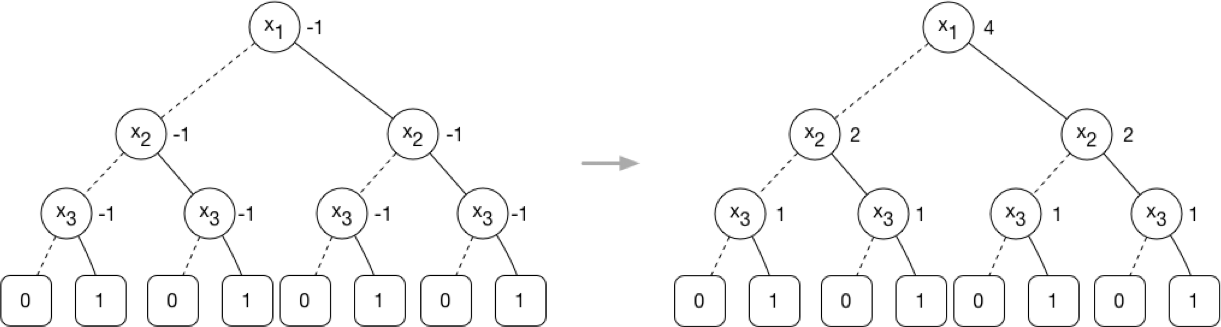
\includegraphics[scale=0.3]{./img/satcount}
	\caption[BDD zur Verdeutlichung der Ermittlung von erfüllenden Belegungen]{BDD zur Verdeutlichung der Ermittlung von erfüllenden Belegungen}
	\label{fig:satcount}
\end{figure}\\
\noindent
Dementsprechend gibt es hierbei vier erfüllende Belegungen für $G$. Hervorzuheben ist, dass -- wenn ein ROBDD vorliegen würde -- natürlich i.\,d.\,R. weniger Kanten passiert werden müssen. Dennoch bleibt die Laufzeit linear in der Größe des BDDs.\\
Bei anderen Darstellungen für Boolesche Funktionen -- bis auf Wahrheitstafeln -- ist die Laufzeit nicht polynomiell beschränkt \cite{m2007}. Bei Wahrheitstafeln gilt ebenfalls eine lineare Laufzeit, wobei hervorzuheben ist, dass sich dort die Platzkomplexität in Grenzen halten muss. So würden bspw. $100$ Variablen in $2^{100}$ Zeilen resultieren, weshalb die Variablenanzahl $n$ nicht zu groß sein darf.
\subsubsection{Tautologietest}
\label{sec:tautologietest}
In der Einleitung auf Seite \pageref{sec:einleitung} wurde erwähnt, dass der Tautologietest mithilfe eines ROBDD in konstanter Zeit möglich ist. Im Folgenden soll dieses Entscheidungsproblem ebenfalls algorithmisch analysiert werden. Ein BDD ist eine Tautologie, gdw. es nur aus einem 1-Blatt besteht:\\
\begin{tabular}{l|p{12cm}}
	\textbf{Eingabe:} & OBDD $G$ für $f \in \mathbb{B}_n$. \\ 
	\textbf{Ausgabe:} & \texttt{JA}, falls $f$ von jeder Belegung erfüllt wird (gültig), \texttt{NEIN} sonst. \\ 
	\textbf{Verfahren:} & Es müssen alle Pfade gesucht werden, die von der Wurzel zu einem 1-Blatt führen. Diese können mithilfe von einem rekursiven Algorithmus berechnet werden, der bei der Wurzel startet. Für jeden inneren Knoten $v$ wird dieselbe Methode für beide Nachfolger sukzessive aufgerufen. Wird ein 1-Blatt erreicht, so wird der Pfad rekonstruiert und die getesteten Variablen derartig belegt, dass dieser Pfad durchlaufen wird.\\
	\textbf{Komplexität:} & $O(|G|)$, da jeder Knoten und jede Kante betrachtet werden muss.
\end{tabular}
Eine Implementierung für das Verfahren kann in Form von Code \ref{lst:checkTautology} folgendermaßen aussehen:
\lstset{language=xml}
\begin{lstlisting}[frame=htrbl, caption={Implementierung von {\ttfamily checkTautology}}, label={lst:checkTautology}]
program checkTautology()
  input: G (in Form eines OBDDs)
  output: Status, ob alle Belegungen zum Wert '1' auswerten
  x := Variablen
  w := Alle Belegungen zu '1'
  if (G = 0) then
    return []
  else if (G = 1) then 
    return [{}]
  else 
    return [{checkTautology(low(G)).add(w.front((map(x[G], 0))))},
      {checkTautology(high(G)).add(w.front((map(x[G], 1))))}]
end program
\end{lstlisting}
Es wird eine Variablenordnung von $\pi : x_1, \dots, x_n$ angenommen. Eine Rückgabe \texttt{\{[]\}} würde z.\,B. bedeuten, dass eine Sequenz mit einer leeren Belegung zur Erfüllung einer Formel zurückgegeben wird.\\
Wenn $G$ jedoch reduziert ist, so muss lediglich geprüft werden, ob die Wurzel von $G$ das 1-Blatt ist. Dies ist trivial und daher in konstanter Laufzeit möglich \cite[S.38]{s2007}. Ein Beispiel hierfür wäre die Boolesche Funktion $f(x_1, x_2, x_3) = x_1 + x_2 + \neg x_1 + x_3$, wobei $f \in \mathbb{B}_3$. Offensichtlich ist diese Funktion eine Tautologie, da das ROBDD lediglich das $1$-Blatt beinhaltet.\\
Im Hinblick auf die Implementierung (siehe Kapitel \ref{sec:ite} auf Seite \pageref{sec:ite}) können durch diese Operation weiterhin zusätzliche ITE-Aufrufe gespart werden, was dort genauer erläutert wird.\\
Im Vergleich zu anderen Darstellungen bleibt zu erwähnen, dass der Tautologietest für Schaltkreise, Boolesche Ausdrücke sowie die DNF nur in exponentieller Zeit entscheidbar ist \cite{m2007}. So müssen z.\,B. für Boolesche Ausdrücke alle $2^n$ Belegungen systematisch erzeugt werden. Für die KNF hingegen ist dieser Test in polynomieller Laufzeit entscheidbar, da diese genau dann nicht erfüllbar ist, wenn sie mindestens eine Klausel enthält.